\begin{frame}{Lower bound. Ideas}

    \begin{theorem}
        Let $G$ be an $(r, \Delta, (1 - \eta) \Delta)$-expander. If
        $\varphi$ is based on $G$ then RCC of $\Search_{\varphi}$ is
        at least $\approx \min(\Delta r, 2^{\Delta})$.
    \end{theorem}

    \pause
    \vspace{0.5cm}
    \begin{itemize}
        \item Decision tree lower bound (tree-like resolution).
            \pause
            \begin{itemize}
                \item \alert{Randomized} lower bound.
            \end{itemize}
            \pause
        \item \only<3>{Lifting?} \pause \sout{Lifting?} \alert{No gadget.}
            \pause
        \item Lifting! Structure vs. randomness.
    \end{itemize}
\end{frame}

\begin{frame}{Decision tree. Expansion}

    \begin{minipage}{0.38\linewidth}
        \centering
        \begin{tikzpicture}

    \pgfmathsetseed{1000007}
    \foreach \i in {0, 1, ..., 4}{
        \node[graph-vert] (b\i) at (1.5, 0.4 * \i + 2.4) {};
    }

    \foreach \i in {0, 1, ..., 4}{
        \node[graph-vert] (c\i) at (1.5, 0.4 * \i - 0.8) {};
    }

    \foreach \i in {0, 1, ..., 8}{
        \node[graph-vert = {LEIorange!80!black}{0.15cm}] (a\i) at (0, 0.4 * \i) {};
    }

    \draw (a3) -- (b1);
    \draw (a3) -- (b2);
    \draw (a3) -- (b3);
    \draw (a4) -- (b3);
    \draw (a4) -- (b4);

    \draw (a3) -- (c1);
    \draw (a3) -- (c2);
    \draw (a3) -- (c3);
    \draw (a4) -- (c3);
    \draw (a4) -- (c4);


    \fill[rounded corners = 3pt, orange, opacity = 0.2] (-0.2, 1) rectangle (0.2, 1.8);
    \draw[rounded corners = 3pt, orange, thick] (-0.2, 1) rectangle (0.2, 1.8);

    \fill[rounded corners = 3pt, blue!80!black, opacity = 0.2] (1.3, 2.6) rectangle (1.7, 4.2);
    \draw[rounded corners = 3pt, blue!80!black, thick] (1.3, 2.6) rectangle (1.7, 4.2);

    \fill[rounded corners = 3pt, blue!80!black, opacity = 0.2] (1.3, 1) rectangle (1.7, -0.6);
    \draw[rounded corners = 3pt, blue!80!black, thick] (1.3, 1) rectangle (1.7, -0.6);


    \node at (-0.4, 1.8) {$S$};
    \node at (2.25, 3.4) {$\mathrm{N}_{X}(S)$};
    \node at (2.25, 0.2) {$\mathrm{N}_{Y}(S)$};
\end{tikzpicture}
    \end{minipage}
    \begin{minipage}{0.58\linewidth}
        \begin{itemize}
            \item $(r, \Delta, c)$-expander;
            \item $\forall S \subseteq L, |S| \le r \Rightarrow$
                \begin{itemize}
                    \item $\mathrm{N}(S) \ge c |S|$;
                \end{itemize}
        \end{itemize}
    \end{minipage}

    \pause

    \vspace{1cm}
    \begin{itemize}
        \item Easy to satisfy small subformulas;
            \pause
        \item Self-healing (closure): $J < \Delta r / 100 \Rightarrow
            \exists I_J \colon$
            \begin{itemize}
                \item $|I_J| < 100 |J_J| / \Delta$;
                \item $G \setminus (I_J \cup J \cup \mathrm{N}(I_J))$
                    is a good expander.
            \end{itemize}
    \end{itemize}

\end{frame}

\begin{frame}{Decision tree. Strategy}

    \begin{itemize}
        \item Idea: any small subformula can be easily satisfied.
    \end{itemize}

    \pause
    \vspace{0.5cm}

    \begin{itemize}
        \item $J \coloneqq \emptyset$, $\rho \coloneqq \emptyset$.
            \pause
        \item Query $x_i$. $J \gets x_i$.
            \pause
        \item If $\rho(x_i) \neq *$ then answer $\rho(x_i)$ else
            answer any $a_i \in \{0, 1\}$, $\rho \gets (x_i = a_i)$.
            \pause
        \item Extend $\rho$ to $\mathrm{N}(I_J)$ such that $I_J$ is
            satisfied.
        \item Remove $I_J, \mathrm{supp}(\rho)$ from $G$.
    \end{itemize}

    \pause
    \vspace{0.5cm}
    \begin{itemize}
        \item Invariant: $G$ is an $(r, \Delta, 0.9 \Delta)$-expander.
    \end{itemize}

\end{frame}


\begin{frame}{Communication. Balanced case [HP 17, FPPR 17, S 24]}
    \begin{minipage}{0.38\linewidth}
        \centering
        \input{pics/graph-expansion-comm.tex}
    \end{minipage}
    \begin{minipage}{0.58\linewidth}
        \begin{itemize}
            \item $(r, \Delta, c)$-expander;
            \item $\forall S \subseteq L, |S| \le r \Rightarrow$
                \begin{itemize}
                    \item $\mathrm{N}_{X}(S) \ge c |S|$;
                    \item $\mathrm{N}_{y}(S) \ge c |S|$.
                \end{itemize}
        \end{itemize}
    \end{minipage}

    \pause
    \begin{itemize}
        \item Partition of variables uniformly at random.
    \end{itemize}
\end{frame}


\begin{frame}{Communication steps}

    \begin{center}
        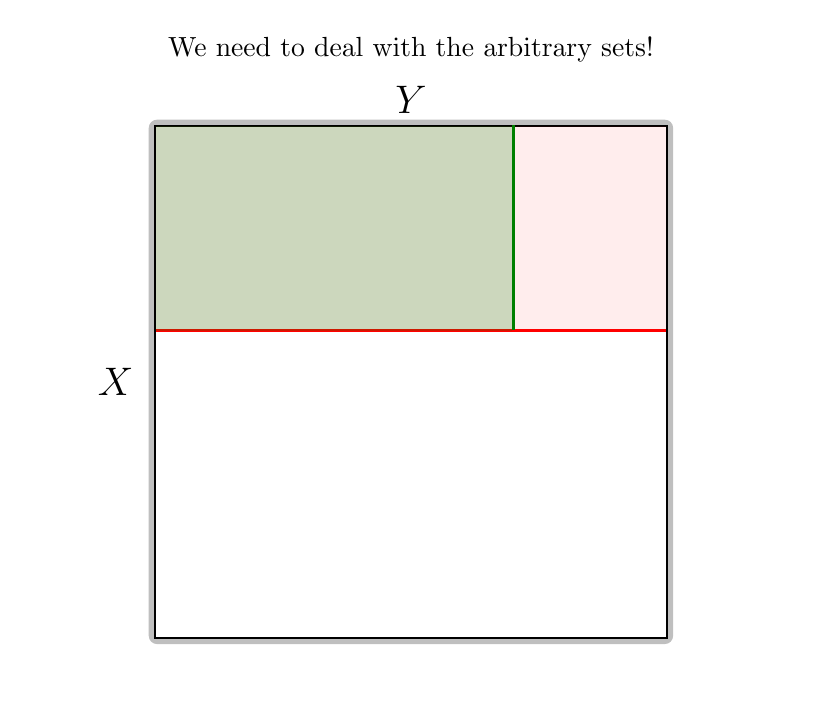
\begin{tikzpicture}
    \def\n{9}
    \def\m{9}
    \def\step{0.65}

    \node at (-1.5, 0) {};
    \node at ({\step * (\m + 1) + 1.5}, 0) {};


    \fill[gray!50, rounded corners = 3pt] (-0.08, 0.08) rectangle
        ({\step * (\n + 1) + 0.08}, {-\step * (\m + 1) - 0.08});
    \fill[white] (0, 0) rectangle ({\step * (\n + 1)}, {-\step * (\m + 1)}); 
    \draw[thick] (0, 0) rectangle ({\step * (\n + 1)}, {-\step * (\m + 1)});
    \node at ({\step * 4}, {-\step * (\m + 1) - 0.56}) {};

    \uncover<2->{
        \draw[very thick, red] (0.01, -4 * \step) --
            ({\step * (\n + 1) - 0.01}, -4 * \step);
    }

    \uncover<3->{
        \fill[red, opacity = 0.07] (0.01, 0) rectangle
            ({\step * (\n + 1) - 0.01}, -4 * \step);
    }

    \uncover<4->{
        \draw[very thick, green!50!black] (7 * \step, 0.01) -- (7 * \step, {-\step * 4 + 0.01});
    }

    \uncover<5->{
        \fill[green!50!black, opacity = 0.2] (0.01, 0) rectangle
            ({\step * 7 - 0.01}, -4 * \step);
    }

    \uncover<6->{
        \node at ({\step * (\m + 1) / 2}, 3 * \step / 2) {\alert{We
                need to deal with the arbitrary sets!}};
    }

 
    \node at (-0.5, {-\step * (\m + 1) / 2}) {\Large $X$};
    \node at ({\step * (\m + 1) / 2}, \step / 2) {\Large $Y$};

\end{tikzpicture}
    \end{center}

\end{frame}

\begin{frame}{Randomness}

    \begin{center}
        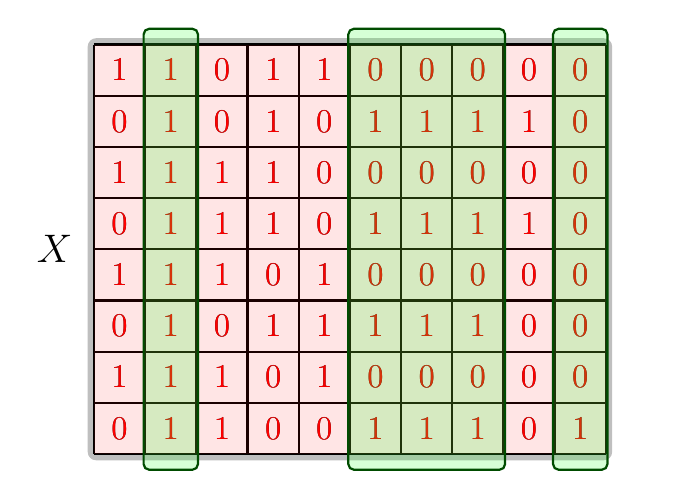
\begin{tikzpicture}
    \def\elements{{
            {1, 1, 0, 1, 1, 0, 0, 0, 0, 0},
            {0, 1, 0, 1, 0, 1, 1, 1, 1, 0},
            {1, 1, 1, 1, 0, 0, 0, 0, 0, 0},
            {0, 1, 1, 1, 0, 1, 1, 1, 1, 0},
            {1, 1, 1, 0, 1, 0, 0, 0, 0, 0},
            {0, 1, 0, 1, 1, 1, 1, 1, 0, 0},
            {1, 1, 1, 0, 1, 0, 0, 0, 0, 0},
            {0, 1, 1, 0, 0, 1, 1, 1, 0, 1}
        }}
    \def\result{{1, 0, 1, 1, 1, 1, 1, 0, 1}} 
    \def\n{9}
    \def\m{7}
    \def\step{0.65}

    \fill[gray!50, rounded corners = 3pt] (-0.08, 0.08) rectangle
        ({\step * (\n + 1) + 0.08}, {-\step * (\m + 1) - 0.08});
    \fill[white] (0, 0) rectangle ({\step * (\n + 1)}, {-\step * (\m + 1)}); 
    \draw[step = \step, thick] (0, 0) grid ({\step * (\n + 1)}, {-\step * (\m + 1)});

    \foreach \i in {0, 1, ..., \n}{
        \foreach \j in {0, 1, ..., \m}{
            \pgfmathparse{\elements[\j][\i]}
            \edef\val{\pgfmathresult}
            \ifthenelse{\val = 0}{
                \node at ({(\i + 0.5) * \step}, {-(\j + 0.5) * \step})
                    {\large \val};
            }{
                \node at ({(\i + 0.5) * \step}, {-(\j + 0.5) * \step})
                    {\textcolor{red}{\large \val}};
                \fill[red, opacity = 0.1]
                    ({\i * \step}, {-\j * \step})
                    rectangle
                    ({(\i + 1) * \step}, {-(\j + 1) * \step});
            }
        }
    }

    \uncover<2->{
        \draw[thick, green!30!black, rounded corners = 2pt, fill = green!80, fill opacity = 0.2]
            ({-0.02 + \step}, 0.2) rectangle ({\step * 2 + 0.02}, {-\step * (\m + 1) - 0.2});
    }

    \uncover<3->{
        \draw[thick, green!30!black, rounded corners = 2pt, fill = green!80, fill opacity = 0.2]
            ({-0.02 + \n * \step}, 0.2) rectangle
            ({(\n + 1) * \step + 0.02}, {-\step * (\m + 1) - 0.2});
    }

    \uncover<4->{
        \draw[thick, green!30!black, rounded corners = 2pt, fill = green!80, fill opacity = 0.2]
            ({-0.02 + 5 * \step}, 0.2) rectangle ({\step * 8 + 0.02}, {-\step * (\m + 1) - 0.2});
    }

 
    \node at (-0.5, {-\step * (\m + 1) / 2}) {\Large $X$};
    \node at ({\step * (\n + 1) + 0.5}, {-\step * (\m + 1) / 2}) {};

\end{tikzpicture}
    \end{center}

\end{frame}

\begin{frame}{Minentropy. $X \subseteq \{0, 1\}^n$}

    \begin{itemize}
        \item Set of coordinates $S \subseteq [n]$ is $\delta$-bad
            $\Leftrightarrow$
            $$
                \exists a \in \{0, 1\}^{|S|},
                \Pr_{x \sim X}[x_{S} = a] \ge
                \left( \frac{1}{2} \right)^{\delta |S|}.
            $$
        \item $X$ is $\delta$-spread iff there are no $\delta$-bad
            sets.
    \end{itemize}

    \pause
    \vspace{0.5cm}
    Fix some $0.9$-spread $X$.
    \begin{itemize}
        \item For any clause with $\Delta$ literals:
            $$
                \Pr_{x \sim X}[C(x) = 0] \le 2^{-0.9 \Delta}.
                        \pause
            $$
        \item Small subformulas of random $\Delta$-CNF are easy to
            satisfy.
            \pause
        \item It was useful for decision trees. Assuming spreadness of
            all sets we are ``done''.
            \pause
        \item $X$ is $\delta$-structured iff bad coordinates are fixed.
    \end{itemize}

\end{frame}


\begin{frame}{Communication. Strategy}

    \begin{itemize}
        \item Split each rectangle into $0.9$-structured rectangles
            (independently for Alice and Bob).
            \pause
        \item Simulate decision tree protocol.
    \end{itemize}

    \pause

    \begin{lemma}
        $\Pi$ is a protocol of depth $d$. There exists a
        structured protocol $\Pi'$ such that:
        $$
            \Pr_{(x, y) \sim U}[\Pi(x, y) \neq \Pi'(x, y)] \le 1 / 100.
        $$
        Moreover for each rectangle in $\Pi'$ there will be at most
        $O(d)$ bad coordinates.
    \end{lemma}

\end{frame}

\begin{frame}{Partition scheme}

    \begin{center}
        \begin{tikzpicture}
    \def\n{9}
    \def\m{9}
    \def\step{0.65}

    \node at (-1.5, 0) {};
    \node at ({\step * (\m + 1) + 1.5}, 0) {};


    \fill[gray!50, rounded corners = 3pt] (-0.08, 0.08) rectangle
        ({\step * (\n + 1) + 0.08}, {-\step * (\m + 1) - 0.08});
    \fill[white] (0, 0) rectangle ({\step * (\n + 1)}, {-\step * (\m + 1)}); 
    \draw[thick] (0, 0) rectangle ({\step * (\n + 1)}, {-\step * (\m + 1)});
    \node at ({\step * 4}, {-\step * (\m + 1) - 0.56}) {};

    \uncover<2->{
        \fill[LEIred, opacity = 0.2] (0, 0) rectangle
            ({\step * (\n + 1) - 0.01}, -4 * \step);
        \draw[very thick, red] (0.01, -4 * \step) --
            ({\step * (\n + 1) - 0.01}, -4 * \step);
        \node at (-0.8, -2 * \step) {$X_{I_1} = a_{I_1}$};

        \node at ({\step * (\n + 1) / 2}, {-\step * (\m + 1) - 0.6})
            {$\Pr[X_{I_j} = a_{I_{j}}] > 2^{0.9 |I_j|}$};
    }

    \uncover<3->{
        \fill[LEIblue, opacity = 0.2] (0, -4 * \step) rectangle
            ({\step * (\n + 1) - 0.01}, -7 * \step);
        \draw[very thick, red] (0.01, -7 * \step) --
            ({\step * (\n + 1) - 0.01}, -7 * \step);
        \node at (-0.8, -5.5 * \step) {$X_{I_2} = a_{I_2}$};
    }

    \uncover<4->{
        \fill[green!50!black, opacity = 0.2] (0, -7 * \step) rectangle
            ({\step * (\n + 1) - 0.01}, -9 * \step);
        \draw[very thick, red] (0.01, -9 * \step) --
            ({\step * (\n + 1) - 0.01}, -9 * \step);
        \node at (-0.8, -8 * \step) {$X_{I_3} = a_{I_3}$};
    }
    
\end{tikzpicture}
    \end{center}
    
\end{frame}